
\documentclass[11pt, a4paper]{article}

% Required packages as per strict LaTeX compilation guidelines
\usepackage[a4paper, margin=2.5cm]{geometry}
\usepackage{amsmath,amssymb,booktabs,array,tabularx,enumitem}
\usepackage{tikz}
\usepackage{booktabs}
\usepackage{enumitem}
\setlist[itemize]{label=-}
\usepackage[hidelinks]{hyperref}
\usepackage{parskip}
\usepackage{graphicx}
\usepackage{float}

\usetikzlibrary{arrows.meta,positioning,calc}

\setlength{\parindent}{0pt}
\setlength{\parskip}{1em}

\begin{document}

% ---------------------------------------------------------
% TITLE PAGE
% ---------------------------------------------------------
\begin{titlepage}
    \centering
    \vspace*{2cm}
    
    {\LARGE \textbf{Lahore University of Management Sciences} \par}
    \vspace{0.5cm}
    {\Large Syed Babar Ali School of Science and Engineering \par}
    
    \vfill
    
    {\Large \textbf{AI651 --- Deep Learning for Space, Time and Graphs} \par}
    \vspace{1cm}
    {\Huge \textbf{Assignment 2 Report} \par}
    
    \vfill
    
    {\Large 
        \textbf{Student Name:} Faaiz Khan \\[0.2cm]
        \textbf{Student ID:} 25280051 
    \par}
    
    \vspace{1.5cm}
    
    % REQUIREMENT: GitHub repository link MUST be on the first page.
    {\large \textbf{GitHub Repository Link:}\\
    \vspace{0.2cm}
    \url{https://github.com/FaaizKhan1999/dl4stg-assignments} \par}
    
    \vspace*{2cm}
\end{titlepage}
% ---------------------------------------------------------

% ---------------------------------------------------------
% TASK 1
% ---------------------------------------------------------
\section*{Question 1 --- River Forecasting Proposal}

A directed river-graph forecaster: each station attends to its upstream sources at learned, state-dependent lags, adds announced releases, and outputs quantiles at S1--S4 for $t_0{+}10,\dots,t_0{+}60$ min.

\subsection*{1.\ Architecture diagram}

$B$ = issuance times, $H{=}72$ history steps, $K{=}6$ horizon steps, $N{=}7$ nodes $\{Q,\mathrm{S1..S4},\mathrm{T1},\mathrm{TU}\}$ ($Q$ = reservoir, TU = virtual node for the unmonitored tributary), $d{=}64$, $\Delta{=}10$\,min.

\begin{figure}[h]
\centering
\resizebox{\textwidth}{!}{%
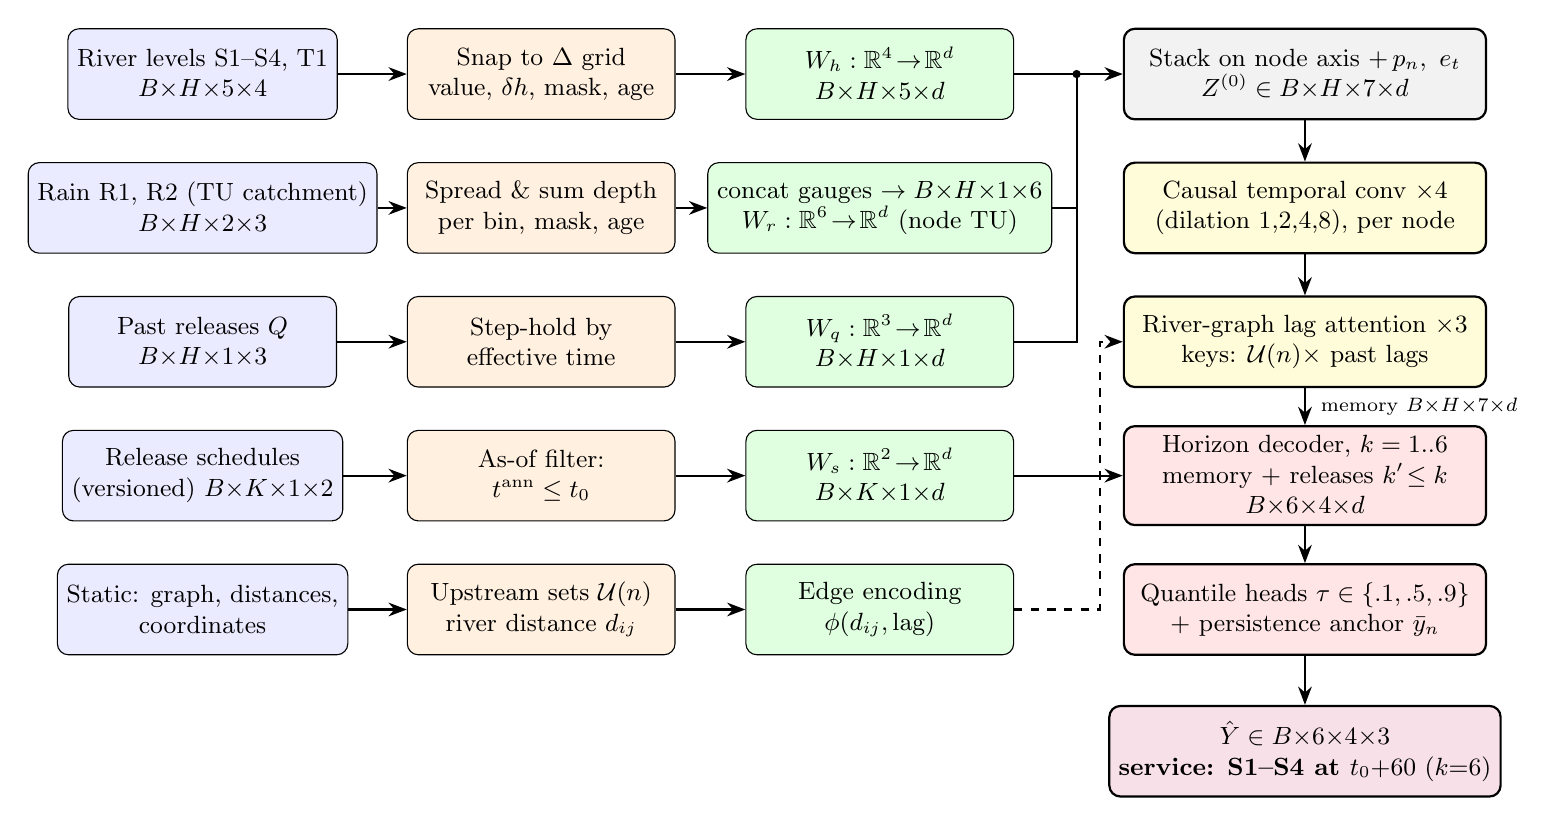
\begin{tikzpicture}[
  font=\small,
  box/.style={draw, rounded corners, align=center, minimum width=3.4cm, minimum height=1.15cm, fill=#1},
  box/.default=white,
  enc/.style={draw, rounded corners, align=center, minimum width=4.6cm, minimum height=1.15cm, fill=#1, thick},
  arr/.style={-{Stealth}, thick},
]
% --- sources
\node[box=blue!8] (h) at (0,0)    {River levels S1--S4, T1\\$B{\times}H{\times}5{\times}4$};
\node[box=blue!8] (r) at (0,-1.7) {Rain R1, R2 (TU catchment)\\$B{\times}H{\times}2{\times}3$};
\node[box=blue!8] (q) at (0,-3.4) {Past releases $Q$\\$B{\times}H{\times}1{\times}3$};
\node[box=blue!8] (s) at (0,-5.1) {Release schedules\\(versioned) $B{\times}K{\times}1{\times}2$};
\node[box=blue!8] (g) at (0,-6.8) {Static: graph, distances,\\coordinates};
% --- alignment
\node[box=orange!12] (ah) at (4.3,0)    {Snap to $\Delta$ grid\\value, $\delta h$, mask, age};
\node[box=orange!12] (ar) at (4.3,-1.7) {Spread \& sum depth\\per bin, mask, age};
\node[box=orange!12] (aq) at (4.3,-3.4) {Step-hold by\\effective time};
\node[box=orange!12] (as) at (4.3,-5.1) {As-of filter:\\$t^{\mathrm{ann}}\le t_0$};
\node[box=orange!12] (ag) at (4.3,-6.8) {Upstream sets $\mathcal U(n)$\\river distance $d_{ij}$};
% --- projection
\node[box=green!12] (ph) at (8.6,0)    {$W_h:\mathbb R^4\!\to\!\mathbb R^d$\\$B{\times}H{\times}5{\times}d$};
\node[box=green!12] (pr) at (8.6,-1.7) {concat gauges $\to B{\times}H{\times}1{\times}6$\\$W_r:\mathbb R^6\!\to\!\mathbb R^d$ (node TU)};
\node[box=green!12] (pq) at (8.6,-3.4) {$W_q:\mathbb R^3\!\to\!\mathbb R^d$\\$B{\times}H{\times}1{\times}d$};
\node[box=green!12] (ps) at (8.6,-5.1) {$W_s:\mathbb R^2\!\to\!\mathbb R^d$\\$B{\times}K{\times}1{\times}d$};
\node[box=green!12] (pg) at (8.6,-6.8) {Edge encoding\\$\phi(d_{ij},\text{lag})$};
% --- encoder / decoder chain
\node[enc=gray!10]   (st)  at (14,0)    {Stack on node axis $+\,p_n,\ e_t$\\$Z^{(0)}\in B{\times}H{\times}7{\times}d$};
\node[enc=yellow!15] (tb)  at (14,-1.7) {Causal temporal conv $\times4$\\(dilation 1,2,4,8), per node};
\node[enc=yellow!15] (ga)  at (14,-3.4) {River-graph lag attention $\times3$\\keys: $\mathcal U(n)\times$ past lags};
\node[enc=red!10]    (dec) at (14,-5.1) {Horizon decoder, $k=1..6$\\memory + releases $k'\!\le k$\\$B{\times}6{\times}4{\times}d$};
\node[enc=red!10]    (hd)  at (14,-6.8) {Quantile heads $\tau\in\{.1,.5,.9\}$\\+ persistence anchor $\bar y_n$};
\node[enc=purple!12] (out) at (14,-8.6) {$\hat Y\in B{\times}6{\times}4{\times}3$\\\textbf{service: S1--S4 at $t_0{+}60$} ($k{=}6$)};
% --- arrows
\foreach \a/\b in {h/ah,r/ar,q/aq,s/as,g/ag,ah/ph,ar/pr,aq/pq,as/ps,ag/pg}{\draw[arr] (\a) -- (\b);}
\draw[arr] (ph) -- (st);
\draw[thick] (pr.east) -| (11.1,0);
\draw[thick] (pq.east) -| (11.1,0);
\fill (11.1,0) circle (1.5pt);
\draw[arr] (ps) -- (dec);
\draw[arr, dashed] (pg.east) -| (11.4,-3.4) -- (ga.west);
\draw[arr] (st) -- (tb);
\draw[arr] (tb) -- (ga);
\draw[arr] (ga) -- node[right, font=\scriptsize, xshift=2pt]{memory $B{\times}H{\times}7{\times}d$} (dec);
\draw[arr] (dec) -- (hd);
\draw[arr] (hd) -- (out);
\end{tikzpicture}}
\caption{Pipeline. Future schedules skip the encoder and enter the decoder on the horizon axis.}
\end{figure}

\begin{figure}[h]
\centering
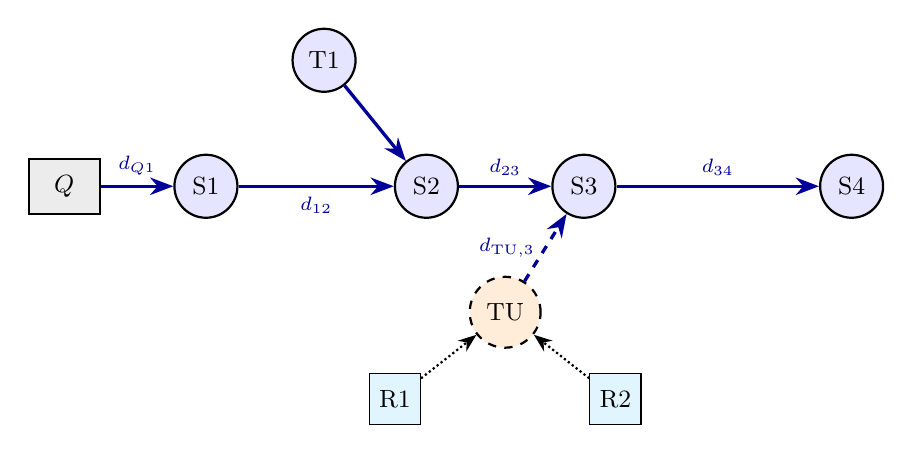
\begin{tikzpicture}[font=\small,
  st/.style={circle, draw, thick, fill=blue!10, minimum size=8mm},
  rg/.style={rectangle, draw, fill=cyan!12, minimum size=6.5mm},
  res/.style={rectangle, draw, thick, fill=gray!15, minimum width=9mm, minimum height=7mm},
  flow/.style={-{Stealth}, very thick, blue!60!black},
  rain/.style={-{Stealth}, densely dotted, thick}]
\node[res] (Q)  at (0,0)    {$Q$};
\node[st]  (S1) at (1.8,0)  {S1};
\node[st]  (S2) at (4.6,0)  {S2};
\node[st]  (S3) at (6.6,0)  {S3};
\node[st]  (S4) at (10,0)   {S4};
\node[st]  (T1) at (3.3,1.6){T1};
\node[circle, draw, thick, dashed, fill=orange!15, minimum size=9mm] (U) at (5.6,-1.6) {TU};
\node[rg]  (R1) at (4.2,-2.7) {R1};
\node[rg]  (R2) at (7.0,-2.7) {R2};
\draw[flow] (Q)  -- node[above]{\scriptsize $d_{Q1}$} (S1);
\draw[flow] (S1) -- node[below]{\scriptsize $d_{12}$} (S2);
\draw[flow] (S2) -- node[above]{\scriptsize $d_{23}$} (S3);
\draw[flow] (S3) -- node[above]{\scriptsize $d_{34}$} (S4);
\draw[flow] (T1) -- (S2);
\draw[flow, dashed] (U) -- node[left, font=\scriptsize]{$d_{\mathrm{TU},3}$} (S3);
\draw[rain] (R1) -- (U);
\draw[rain] (R2) -- (U);
\end{tikzpicture}
\caption{River graph. Solid: river edges with distances. Dotted: rain gauges feed only the virtual node TU (A7). $\mathcal U(n)$ = $n$ plus every node with a path into $n$.}
\end{figure}

\subsection*{2.\ Assumptions}

\textbf{Supplied facts:} 10-min levels at S1--S4 and T1; timestamped rain at R1, R2; recorded releases and schedules with announcement and effective times; topology and river distances. Travel times and unmonitored inflow are not supplied; future rain and levels are unavailable at issuance.

\begin{enumerate}[label=\textbf{A\arabic*}, leftmargin=*, itemsep=0pt]
  \item $\ge$3 years of data including several floods, so high-flow behaviour can be learned.
  \item Levels arrive within $\sim$20 min and rain within $\sim$30 min, with arrival times logged, so inputs can be built from what had actually arrived.
  \item Gaps are short and occasional, and faulty readings are detectable by range and rate checks, so masking is enough.
  \item Each rain report gives the depth since the previous report, so rain is summed per bin rather than interpolated.
  \item Everything relevant to a 1-h forecast occurred within the last 12\,h, which sets $H{=}72$.
  \item Flow is downstream only (no backwater), so stations attend only upstream.
  \item R1 and R2 flank the unmonitored tributary's catchment (map), so rain enters the model only through TU and affects only S3 and S4. Rain elsewhere is either buffered by the reservoir (reaching S1 via releases) or already visible in T1's levels.
  \item Unmonitored inflow is mainly rain-driven, so R1 and R2 are usable proxies for it.
  \item Travel time varies smoothly with flow and distance on a stable channel, so learned lags generalise.
  \item Release records are accurate and schedule versions are archived, which is needed for leak-free training.
  \item Each station has a fixed level datum, so the model can predict change from the last level.
  \item Future rain is unknown, so it is represented as uncertainty rather than as an input.
\end{enumerate}

\subsection*{3.\ Forecasting task and data specification}

\[
\mathcal I(t_0)=\{r: t^{\mathrm{obs}}_r\le t_0,\ t^{\mathrm{arr}}_r\le t_0\}\cup\{\text{schedules with } t^{\mathrm{ann}}\le t_0\},
\]
\[
\text{history } j=-71..0\ (12\text{\,h}),\qquad \text{horizon } k=1..6\ \ (k{=}6:\ t_0{+}60\text{ min}).
\]
Forecasts are issued every 10 min at $t_0$ using only $\mathcal I(t_0)$. The outputs are the quantiles $\tau\in\{0.1,0.5,0.9\}$ of the level at S1--S4.

\begin{center}\small
\begin{tabularx}{\textwidth}{@{}l l X l@{}}
\toprule
Tensor & Dims & Axes / features & Coverage\\
\midrule
$X^h$ levels & $B{\times}H{\times}5{\times}4$ & batch, time, node (S1--S4, T1); [level, $\delta h$, mask, age] & $(t_0{-}12\text{h},t_0]$\\
$X^r$ rain & $B{\times}H{\times}2{\times}3$ & batch, time, gauge; [$\log(1{+}\text{depth})$, mask, age]; reshaped to $B{\times}H{\times}1{\times}6$ as TU's features & $(t_0{-}12\text{h},t_0]$\\
$X^q$ past releases & $B{\times}H{\times}1{\times}3$ & batch, time, $Q$; [actual, scheduled as-of, mask] & $(t_0{-}12\text{h},t_0]$\\
$X^s$ schedule & $B{\times}K{\times}1{\times}2$ & batch, horizon, $Q$; [release, available] & $(t_0,t_0{+}1\text{h}]$, $t^{\mathrm{ann}}{\le}t_0$\\
$P$; $D,M$ & $N{\times}F_p$; $N{\times}N$ & node static features; distances, upstream mask & static\\
$Y$, $m$ & $B{\times}K{\times}4$ & batch, horizon, station; target, observed-mask & $t_0{+}k\Delta$\\
$\hat Y$ & $B{\times}K{\times}4{\times}3$ & batch, horizon, station, quantile & issued at $t_0$\\
\bottomrule
\end{tabularx}
\end{center}

\textbf{Alignment.}
\begin{itemize}[leftmargin=*, itemsep=0pt]
  \item \emph{Time:} levels take the last value in each 10-min bin; rain depth is spread over its report interval and summed per bin; releases are step-held. Masks and ages mark gaps.
  \item \emph{Space:} sources are not interpolated. Each source is a node, except that the two gauges are concatenated into TU. Nodes relate only through $\mathcal U(n)$ and $d_{ij}$.
  \item \emph{Features:} per-type projections $W_c$ map every source to width $d$ before stacking on the node axis.
\end{itemize}

\subsection*{4.\ Model computations and design justification}

Notation: $\mathcal U(n)$ = upstream closure (Fig.~2), e.g.\ $\mathcal U(\mathrm{S3})=\{\mathrm{S3},\mathrm{S2},\mathrm{S1},\mathrm{T1},Q,\mathrm{TU}\}$ and $\mathcal U(\mathrm{S2})=\{\mathrm{S2},\mathrm{S1},\mathrm{T1},Q\}$; $h_{t,n}\in\mathbb R^d$ is the representation of node $n$ at time $t$.

\noindent One this to note is that TU has no measurements, so $h_{t,\mathrm{TU}}$ is a learned rain feature, not an inflow estimate. It could be tied to actual inflow only through a constraint (e.g.\ on S3's rise relative to S2) or a future tributary gauge; with a gauge, TU becomes a supervised node with no structural change.
\begin{table}[H]
\centering
\renewcommand{\arraystretch}{1.8}
\resizebox{\linewidth}{!}{%
\begin{tabular}{@{}ll@{}}
\toprule
\textbf{Stage} & \textbf{Formulation} \\
\midrule
(a) Projection &
$z^{(0)}_{t,n}=W_{c(n)}x_{t,n}+p_n+e_t$ \\
(b) Temporal &
$h^{(\ell)}_{t,n}=h^{(\ell-1)}_{t,n}+\mathrm{MLP}\big(\sum_{j=0}^{2}W_j h^{(\ell-1)}_{t-j\delta_\ell,n}\big),\quad \delta_\ell=1,2,4,8$ \\
(c) Lag attention &
$\begin{aligned}
&\alpha_{t,j}(i,s)=\operatorname{softmax}_{i\in\mathcal U(j),\,s\le t}\tfrac{(W_Qh_{t,j})^{\top}(W_Kh_{s,i}+\phi(d_{ij},t{-}s))}{\sqrt d}\\
&h_{t,j}\mathrel{+}=\textstyle\sum_{i,s}\alpha_{t,j}(i,s)\,W_Vh_{s,i}
\end{aligned}$ \\
(d) Decoder &
$u_{k,n}\mathrel{+}=\mathrm{Attn}\big(u_{k,n};\{h_{s,i}:i\in\mathcal U(n)\}\cup\{f_{k'}:k'\le k\}\big),\quad f_{k'}=W_sx^s_{k'}+e_{k'}$ \\
(e) Output &
$\hat y^{(0.5)}_{k,n}=\bar y_n+\sigma_n a,\quad \hat y^{(0.9)}=\hat y^{(0.5)}+\sigma_n\,\mathrm{softplus}(b),\quad \hat y^{(0.1)}=\hat y^{(0.5)}-\sigma_n\,\mathrm{softplus}(c)$ \\
(f) Loss &
$\displaystyle \mathcal L=\frac{\sum w_b\,m\,\rho_\tau(y-\hat y^{(\tau)})}{\sum w_b\,m},\quad \rho_\tau(r)=\max(\tau r,(\tau{-}1)r),\quad w_b=1+\lambda\,\mathbb 1[\text{flood}]$ \\
\bottomrule
\end{tabular}}
\caption{Model components.}
\label{tab:model}
\end{table}

\noindent\textbf{Why each block:}
\begin{itemize}[leftmargin=*, itemsep=0pt]
  \item[(b)] Captures local trends and rain-accumulation shape.
  \item[(c)] One layer reaches every upstream source at every lag (A5). The query and key depend on the current states, so lags shift with flow (A9). $\phi$ handles uneven spacing. $\mathcal U$ encodes flow direction (A6).
  \item[(d)] Lets announced releases act on the forecast, but only on steps where they are already effective ($k'\le k$).
  \item[(e)] Anchoring on the last level $\bar y_n$ means the model predicts change from persistence (A11). Softplus increments keep the quantiles from crossing.
  \item[(f)] A point loss returns only the mean (MSE) or median (MAE). The irreducible uncertainty from the tributary and future rain needs bands, and $w_b$ up-weights floods.
\end{itemize}
Training uses chronological splits, as-of inputs, random masking, a 5-seed ensemble and conformal calibration.

\begin{center}\small
\begin{tabularx}{\textwidth}{@{}l X@{}}
\toprule
Source & Path to the forecast\\
\midrule
Upstream stations & Keys in downstream lag attention (c), read at state-dependent lags\\
T1 & In $\mathcal U$(S2, S3, S4); contribution learned\\
Rainfall & R1, R2 $\to$ TU (a, b); TU is a key for S3 and S4 only (c), at a learned catchment-plus-travel lag (A7, A8)\\
Releases & Past: via $Q$ in (c). Announced future: decoder (d), mainly affecting S1\\
\midrule
\textbf{Imposed (physical)} & Topology and direction; causality ($s{\le}t$, $k'{\le}k$, no future rain); distances; rain acts only via TU; rain as depth; level continuity\\
\textbf{Learned} & Travel times, attenuation, confluence mixing, rain $\to$ TU $\to$ S3 response, release response, band widths\\
\bottomrule
\end{tabularx}
\end{center}

\subsection*{5.\ Operation and exceptional conditions}

\begin{center}\small
\begin{tabularx}{\textwidth}{@{}l X@{}}
\toprule
Condition & Handling\\
\midrule
(i) Missing & Value $\to$ 0 with mask $=1$ and growing age; $\bar y_n$ uses the last valid level. Training randomly drops points, blocks and whole stations. Missing targets are masked out of the loss. If all river data fail, fall back to persistence and alert.\\
(ii) Delayed & Only records with $t^{\mathrm{arr}}\le t_0$ are used; a late record counts as missing until it arrives and is used in the next 10-min cycle. Training replays history as-of each issuance with logged delays (A2).\\
(iii) Announced releases & Latest schedule with $t^{\mathrm{ann}}\le t_0$, step-held onto $k=1..6$. Training uses archived versions, never actual future releases (that would be leakage).\\
(iv) Scheduled $\ne$ actual & The past input holds both actual and as-of scheduled releases, so the model learns how far to trust schedules. A live deviation appears through $Q$ within one cycle. Optional $\pm20\%$ release scenarios.\\
\bottomrule
\end{tabularx}
\end{center}

\noindent\textbf{Feasibility.} With $L=HN=504$ tokens, even dense attention costs $2L^2d\approx3\times10^7$ MACs per layer, about $10^9$ for the full 5-member ensemble. That is under 1\,s on a CPU, so ingestion dominates the 10-min cycle.

\subsection*{6.\ Uncertainty, limitations and additional information}

Uncertainty is reported as calibrated 10--90\% bands (quantiles, ensemble spread and conformal calibration).

\begin{center}\small
\begin{tabularx}{\textwidth}{@{}>{\raggedright\arraybackslash}p{2.9cm} X X@{}}
\toprule
Limitation & Impact & Response / unresolved\\
\midrule
Unmonitored tributary & Unexplained rises at S3, S4 & TU rain proxy, wider bands; storms missing both gauges unresolved\\
Changing travel times & Timing errors on rising limb & State-dependent lags; floods beyond record unresolved\\
No future rain & Fast rises under-forecast & Bands widen after rain; needs nowcasts\\
Rain elsewhere unmeasured (local runoff S2--S4, T1 and S1 catchments) & Sudden local rises seen only once they reach a station & Level histories, wider bands; largely unresolved\\
Few extremes, drift & Peaks under-estimated & Event weighting, monitoring, retraining\\
Schedule deviations & Errors at S1, S2 & Deviation input, 10-min refresh\\
Sensor faults & Corrupted inputs and targets & QC and masks; slow drift partly unresolved\\
\bottomrule
\end{tabularx}
\end{center}

\begin{center}\small
\begin{tabularx}{\textwidth}{@{}>{\raggedright\arraybackslash}p{4.2cm} X >{\raggedright\arraybackslash}p{2.6cm}@{}}
\toprule
Request & Benefit & Usable without?\\
\midrule
Gauge on unmonitored tributary & Supervises TU; removes the largest S3/S4 error & Yes (rain proxy)\\
Rain gauges on T1 catchment and main-river reach & Earlier warning of local runoff & Yes\\
Rain radar / nowcasts & Future-rain input & Yes, wider bands\\
Travel-time studies & Lag prior for $\phi$; validation & Yes\\
Rating curves, flood thresholds & Discharge checks, warning levels & Yes\\
Telemetry delay and QC logs & Realistic delay simulation & Yes (A2, A3)\\
Archived schedule versions & Leak-free training & Partly (lower skill)\\
Reservoir operating rules & Anticipate unscheduled releases & Yes\\
\bottomrule
\end{tabularx}
\end{center}


% ---------------------------------------------------------
% GENERATIVE AI USAGE (MANDATORY SECTION)
% ---------------------------------------------------------
\section*{Generative AI Usage}

\textit{Generative AI tools were utilized during the completion of this assignment strictly as supplementary assistants. Primarily, AI was used as a learning aid to deepen my understanding of the assignment's underlying concepts, as well as to break down the specific architectures and techniques required for the tasks.} 

\textit{Furthermore, these tools provided support in the drafting and grammatical refinement of this report, debugging and structuring programming code, and compiling supporting evidence. However, all core ideas, critical analyses, experimental methodologies, and final implementations presented in this document are entirely my own original work. The AI was leveraged to facilitate execution and conceptual clarity, not to replace independent critical thinking or problem-solving.}

\end{document}

